\documentclass[]{report} % Import report.cls
% ----------------------------------------------------------------------------

% Document Encodings
\usepackage[english]{babel}
\usepackage[utf8]{inputenc}
\usepackage[T1]{fontenc}

% Graphics
\usepackage{graphicx}
\usepackage[section]{placeins}
\graphicspath{{./imgs/}}

% Mathematic Symbols
\usepackage{amsthm, amsmath, amssymb, amsfonts, bbm, mathrsfs }

%bibliography
\usepackage[square,numbers]{natbib}
\usepackage[nottoc]{tocbibind} % reference in table of contents
\bibliographystyle{abbrvnat}

\usepackage{caption, subcaption} % figure captions
\usepackage{listings}
\lstset{
	language=Python,
	frame=single,
	label={lst:params}
}

% Miscellaneous
\usepackage{setspace} % For using single or double spacing
\usepackage{fancyhdr} % For the headers
\usepackage{longtable} % Tables that can span several pages
\usepackage{hyperref} % Adds clickable links at references


% Hide chapter Numbers
\usepackage{titlesec}
\titleformat{\chapter}[display] {\Large\bfseries\centering} {} {1pt} {\huge }           % before-code

% ----------------------------------------------------------------------------
% Begin Document
% ----------------------------------------------------------------------------
\begin{document}

\pagestyle{empty}
\frontmatter % Use roman page numbering  ( i,ii, iii, ... )

% Project Title
% ............................................................................
\begin{titlepage}
	\begin{center}
		\vfill
		
		%{\huge \scshape Kiel University of Applied Science }\\[0.5cm]
		%\rule{\textwidth}{1pt}\\[0cm]
		
		% FH LOGO
		% ---------------------------------
		%\FloatBarrier
		\begin{figure}[h]
			\centering \includegraphics[width=\textwidth]{fh_kiel_logo.png}
		\end{figure}
		%\FloatBarrier
		\rule{\textwidth}{1pt}\\[0cm]
		% ---------------------------------
		
		\center \huge{MS. Information Engineering(MIE), IuE}
		
		\vspace*{1.5\baselineskip}
		
		\center \Large{ \textbf{Date:} 05 August 2024}\\[1.0cm]
		
		\rule{\textwidth}{0.5pt}\\[0cm]
		{\huge \bfseries {Training Prosumer Agents with Reinforcement Learning for Energy and Cost Optimization } \par \ }\\[-0.5cm]
		\rule{\textwidth}{1.5pt}\\[1cm]
		
		\center \Large{ \textbf{\underline{In cooperation with}} \\[0.3cm] Forschungsstelle für Energiewirtschaft e. V.}\\[1.5cm]
		
		\hfill \large \textbf{\underline{Submitted by}}\\[0.3cm] \hfill
		\hfill  {\large \text{Sudesh Acharya}}\\ [0.1cm]
		\hfill  {\large{Mat. Nr. : 932253}}\\ [1.5cm]
		
		\hfill \large \textbf{\underline{Under the Supervison of}}\\[0.3cm]
		\hfill  {\large \text{Prof. Dr. Hauke Schramm}}\\ [0.1cm]
		\hfill  {\large \text{Mr. Vincenz Regener(FfE e.V.)}}\\ [0.1cm]
		
		
	\end{center}
\end{titlepage}

\begin{titlepage}
	\begin{center}
		\vspace*{\fill}
		{\large \textit{Submitted as Master Thesiswork for the partial fulfillment of M.S. in Information Engineering, IuE, University of Applied Science, Kiel}}\\[1cm]
		\vspace*{\fill}
	\end{center}
\end{titlepage}

% Blank page
\shipout\null \stepcounter{page}

% Preambles
% ............................................................................
\startpreamble


\unnumberedchapter{Abstract}
\chapter*{ \centering Abstract} 

\vspace*{5\baselineskip}

\begin{large}
\centering
% ............................................................................
\textit{Energy management within private household has seen significant progress in recent years due to the advancement in technology, increasing integration of solar energy generation and adoption of Electric Vehicles(EVs) operating bidirectionally to exchange power. This creates opportunities for a household to participate in energy market by utilizing local and mobile energy assets. This research and development undertaking explores a case of energy management within household by utilizing Reinforcement Learning(RL) methods to learn strategies to minimize net energy exchange cost to the grid.}

\vspace*{1\baselineskip}

\textit{With the use of several RL algorithms and rule based heuristic, this work compares performance of different learned strategies and demonstrates that the agent learns to optimize the objective of cost reduction by a significant margin compared to rule based strategies.}

% ............................................................................
\end{large}



\unnumberedchapter{Acknowledgement}

\chapter*{\centering Acknowledgment}

\vspace*{4\baselineskip}

\begin{large}
% ............................................................................
I would like to express my sincere gratitude to \textbf{Prof. Dr. Hauke Schramm}, for the supervision, guidance, and support. \\

I gratefully acknowledge the invaluable time, supervision, constant encouragement of \textbf{Mr. Vincenz Regener} and \textbf{Mr. Theodor Haug} throughout this undertaking. \\


Also, I greatly appreciate the opportunity from \textbf{Forschungsstelle für Energiewirtschaft e. V.} for letting me in on this exciting project.\\

Last, but not least, i would like to thank \textbf{ University of Applied Science, Kiel} for great learning experience 
through this compulsory Thesiswork. \\
% ............................................................................
\end{large}
	




 

% Table of Contents
% .................................... ........................................
\unnumberedchapter{Contents}
\tableofcontents % Write out the Table of Contents


% Contents
% ............................................................................
\addtocontents{toc}{\vspace{2em}}
\mainmatter % Begin numeric page numbering ( 1, 2, ... )

\chapter{Introduction}\label{ch-1}
% ------------------------------------------------------------------------------------
% Introduction
% ------------------------------------------------------------------------------------

\begin{large}
% ............................................................................

\section{Background}

In recent years, due to increasing adoption of renewable energy sources and awareness of it's impact on mitigation of issues caused by climate change, industries and households are transforming towards climate neutrality. United efforts of countries around the world such as Paris Climate Agreement\cite{parisagreement}(PCA), signed by $195$ countries, to deal with climate change issues, define collective and national goals in short and long terms. Main goals of the PCA agreement include reduction of average global temperature below $2^\circ C$, transparency on progress, awareness programs, and regular assessment of the united goals. Climate Neutral Act \cite{climateact} defines goal to achieve green house gas neutrality by 2050 for Germany, enforcing threshold on permissible emission of $CO_{2}$ on sectors such as energy, transport, and other industries. The energy industry is progressively transitioning from conventional to renewable energy sources in Germany as indicated by the positive trend in figure \ref{fig:energy_gen_de}\\

\begin{figure}[h]
	\begin{center}
		\includegraphics[width=0.9\textwidth]{analytics/energy_gen_per_year.png}
		\caption{\textit{Energy generation in Germany per year [2002-2023]} src:\cite{energychartsinfo} }
		\label{fig:energy_gen_de}
	\end{center}
\end{figure}


This trend is reflected in increasing adoption and integration of renewable sources of energy within households. Traditionally household demand were met solely from the grid, which depended mostly on the generation of energy from conventional sources. With the integration Photo Voltaics(PV), households are not only able to meet partial demand by relying on self-generated energy, but are also able to participate in market by feeding excess back to the grid. These household with bidirectional power exchange to the grid are termed as Prosumers(consumer-producer).

The concept of Prosumer household introduced shift in some responsibility of energy management from centralized distribution hubs to the end user, resulting in Energy Management System(EMS) within Household. The term EMS was first pointed out during the rise of personal computing platform\cite{sems}. Home Energy Management System(HEMS) includes sensing, monitoring, communication and control of load consumption, generated PV, and Energy Storage Systems(ESS) in order to optimize user defined objectives such as minimization of net energy cost, reduced grid dependency, comfort, and emission minimization. \\

Electric Vehicles(EVs), in recent years, has been increasingly integrated within HEMS. \cite{evess} Proposes HEMS integrated with PV, EV and ESS with excess grid feed back. EVs with bidirectional power flow in Electric Vehicles Supply Equipment(EVSE) allows the EVs to be used as a distributed energy storage asset and brings forth opportunities and application for energy exchange to household, participation in grid demand response and energy consumption optimization. \\


Conventionally HEMS were used in the form of analytics and visualization, making the user aware of their consumption and thereby aiding conscious use of household appliances and perform manual scheduling. Rule based scheduling were adopted to include optimization based on pre-defined criteria and thresholds to partially automate control. With advancement in technology, optimization based techniques such as Linear programming(LP) and Mixed Integer Linear Programming(MILP) methods were used to find the best outcome in a scenario, such as optimization of energy consumption and production under constraints like battery capacity and grid limitations. \cite{milp} Utilizes MILP to reduce dissatisfaction and cost of consumers considering EES and Plug-In EVs(PEV). Recent approaches include Dynamic Programming(DP) for optimization objectives such as charging and scheduling strategies based on sequential decision-making. \cite{dphev} Demonstrates a case study on optimization of rule-based strategies in Hybrid Elecric Vehicles(HEV) using DP. Model Predictive Control(MPC), use modeling, prediction of future dynamics, and suggest control strategies. Rule-based approaches often lack adaptability and may not capture complex dynamics. Optimization methods require accurate modeling of dynamics of the system and can be computationally expensive. While MPC approaches offer promising results, they often require large datasets and may not generalize well to unseen scenarios.

RL offers a unique advantage in directly learning optimal control strategies through trial and error, interaction with the environment, making it suitable for handling real-time decision making under uncertainty. \cite{qlearning} uses Q-Learning based scheduling and control of HEMS component with ESS charging and discharging to reduce consumption cost while maintaining user comfort. \cite{drlgym} Provides optimized control method using RL with distributed flexible assets within private households and provides a practitioner guide on implementing such a system. \\ 

\section{Objective}

Optimizing energy flow between the HEMS components while considering dynamic pricing, varying solar generation, distributed and local energy storage system remains a significant challenge. This undertaking focuses on an application domain of a household environment in Germany, integrated with Photo Voltaic(PV) energy generation and energy storage system, exchanging energy with the grid to meet household demand under variable exchange tarrifs(Eur/Kwh). A bidirectional power transfer to and from the energy storage as control action, with the objective of reducing the net exchange cost to a grid by learning useful control strategies using Deep Reinforcement Learning(DRL). \\

\section{Research Questions}

With the objective of learning useful strategies for reduction of net exchange energy cost within a household, several research question were explored. This includes the possibility of modeling of HEMS control system as a Prosumer RL Agent, impact of selection of algorithm on performance of the system and factors influencing the learned strategies by an Agent. Following list outlines the question more concretely. 

\begin{itemize}
	\item How can Prosumer Agents be modeled in a  Reinforcement Learning
		environment?
	\item Can RL effectively minimize cost of energy under time-variable tarrifs ?
	\item How does the choice of RL algorithm impact  performance of the control system ?
	\item What are the key factors influencing the optimal control strategies learned by the RL agent?
\end{itemize}

Within the scope of addressing these questions and optimizing the objective, remainder of the document is organized as follows. Section \ref{ch-2} describes methodology and underlying theoretical framework based on defined objectives. Section \ref{ch-3} describes different components involved in development of experimentation framework to model, test and collect observations. Section \ref{ch-4} explores the resulting observation, their interpretation and relevance on answering the research questions. Final Section \ref{ch-5} compares and contrasts on the objective and the achieved outcomes. \\

%............................................................................
\end{large}


\numberedchapter

\chapter{Methodology} \label{ch-2}

\begin{large}
	
This section describes the components and methodologies used to achieve the objectives defined in previous section. Since the chosen methodology is based on RL, which is a data-driven method that learns control action directly from the datasets using Deep Neural Networks(DNNs). It begins with descriptive analytics of dataset in use. The subsection following describes foundations and concepts of theoretical framework in use. The RL based framework requires trial and error learning, therefore there is need of implementation of custom environment simulating HEMS. The simulated environment and its different types, based on their involvement in steps of modeling are discussed. A reward function definition/design is crucial part of the setup to learn policy as the reward reinforcement dictates the behavior(action under given policy) of an agent. Finally appropriate algorithms are selected for the learning of the policy itself. \\ 


\section{Data Description}

Since the modeling of policy network or deep neural networks in general, is based direct mapping of data to resulting unit(action), it is important to select input observation/features to be representative of information needed by agent to make decisions. The dataset \cite{dataset} provided is an open dataset on residential bidirectional EV charging. It includes roughly a year of time series dataset with 15 minutes resolution, collected in private customer household in southern germany. The dataset includes power monitoring at Grid Connected Point(GCP) with positive values, generated PV power with negative values and power through bidirectional Electric Vehicle Supply Equipment(EVSE) as positive values. Power drawn by a household ($P_{HH}$) is derived as $P_{HH}=P_{GCP}-P_{PV}-P_{EVSE}$. It further includes information on EV such as boolean connection status, current State of Charge(SoC) of the EV and target SoC(SoC level to attain with user pre-defined departure time). Although the dataset is useful for many scenarios such as EV power exchange to Household, Grid, other Energy consumption devices, for the use case at hand, only the information on Power consumed from grid to meet household demand ($P_{HH}$), power of generated PV($P_{PV}$) is utilized. The unit of Power is measured in Watts. Additional time series dataset\cite{energychartsinfo} on day ahead variable energy exchange price of hourly resolution is utilized. \\

Further description of data is projected as distribution of samples for each selected features as shown in figure \ref{fig:dev_datainfo}. The distribution of sample values in Power PV data is shown in the upper left section of the figure. As discussed in the data collection process\cite{dataset}, the data values of ($P_{PV}$) is always below $0$. Around $64\%$ of the sample values lie within $(-0.5, 0)$ with average value of $-1.789$. Similarly, in the upper right section of the figure represents distribution of values for Power Household with $71\%$ of value within $(0, 0.5)$. These ($P_{HH}$) value have mean of $0.542$ and always lie above $0$. Auction price data is a near normal distribution with mean value of ($0.192$). These statistics could provide some insights on impact of set of these observation input values on resulting action of the Agent. \\


\begin{figure}[h]
	\begin{center}
		\includegraphics[width=0.9\textwidth]{development/input_distributions.png}
		\caption{ \textit{Data distribution of observation inputs} }
		\label{fig:dev_datainfo}
	\end{center}
\end{figure}

While distribution may provide information on individual samples, it fails to represent the temporal relationship among them. Upon additive decomposing, the data series can be visualized in terms of component such as Trend(T), Seasonality(S) and Residuals( i.e. $\text{Time Series}=T+S+R$). The Repetition of patterns of behaviors in household consumption and PV generation, reflected on different scale of time range are termed as seasonality. The trend component can be interpreted as margin of consecutive values over period of time or patterns without seasonal component. The residual part of the series, as the name suggests, is rest of the composition after reducing patterns of trend and seasonality. \\

Figures \ref{fig:dev_input_decompose_daily} and \ref{fig:dev_input_decompose_hourly} show decomposition of input observation series for a day in a week and hour in a day respectively. There are several scales of patterns that can be identified through the full range of dataset length such as season or months of the year with variation in PV generation, price of energy. Yearly and Monthly decomposition is limited by size of dataset. Selection of time frame window as day in a week allows us to see and compare daily pattern in consumption shown in blue graph in upper left section. It starts with Friday with heavy consumption pattern during morning and evening hours, higher during weekends and average for the rest of the weekdays. A trend in increase in auction price can be seen during weekdays and reduced in weekend likely reflection of less demand from industries.  \\

\begin{figure}[h]
	\begin{center}
		\includegraphics[width=0.9\textwidth]{development/input_daily_decomposition.png}
		\caption{ \textit{Additive decomposition of observation inputs (daily)}}
		\label{fig:dev_input_decompose_daily}
	\end{center}
\end{figure}

Since the PV patterns are independent of weekdays, an hourly decomposition in a day was selected as shown by the green curve. The PV peaks during mid-day when the sun is up, household demand is less during work hours. \\

\begin{figure}[h]
	\begin{center}
		\includegraphics[width=0.9\textwidth]{development/input_hourly_decomposition.png}
		\caption{ \textit{Additive decomposition of observation inputs (hourly)} }
		\label{fig:dev_input_decompose_hourly}
	\end{center}
\end{figure}

The description of different properties of dataset such as sample distributions, seasonal and trend components decomposition could allow interpretation of the pattern in agents behavior later during inference, since these input series solely are used to learn policies. The residual part is distinguished from other component and may represent important information whereas seasonality and trend might introduce fluctuations. \\

\section{Theoretical Framework}

Main concept of reinforcement learning (RL) revolves around an agent learning to make decisions in an environment through trial and error, with the goal of maximizing a reward. A typical agent environment interaction\cite{rlintro} is shown in the figure \ref{fig:fmdp}. The main components and terminologies of such interactions are described as follows.\\


\begin{figure}[h]
	\begin{center}
		\includegraphics[width=0.8\textwidth]{components/finite_mdp.png}
		\caption{ \textit{Agent environment interaction}}
		\label{fig:fmdp}
	\end{center}
\end{figure}


\begin{itemize}
	\item{\textbf{Environment}: It is the world or system the agent operates in. It provides the agent with feedback in the form of rewards or penalties based on its actions.}
	\item{\textbf{State}: It represents the current situation in the environment relevant to the agent's decision-making. Special states are initial and termination states}
	\item{\textbf{Reward}: It is a numerical value assigned to the agent after it takes an action. Positive rewards indicate good choices, while negative rewards indicate bad choices. The reward function guides the agent's learning by shaping its understanding of what actions lead to intended behavior.}
	\item{\textbf{Policy}: It is the strategy the agent uses to map states to actions. Through trial and error, the agent learns and refines its policy to make better decisions in the future. The cycle of action, reward, and policy update continues as the agent learns through experience until some termination or truncation criteria is met.}
	\item{\textbf{Action}: It is what the agent chooses to do in a particular state under current policy/rule.}
\end{itemize}

A RL system in context of HEMS with finite set of observation states is based on a decision process termed as Markov Decision Process(MDP) and is defined in terms of tuple $(S, A, P, R, \gamma)$. where, $S$ is set of all possible permutation of observation values, $A$ is set of all possible action taken by decision making agent, $P$ is state transition probability matrix $P_{ss^{'}}^{a}$ as state transition to future state $S_{t+1}$, given current state $S_t$ for current action, i.e. $P_{ss^{'}} = \mathbb{P}[S_{t+1} = s^{'} | S_t = s]$, $R$ is estimated return $R_{s}^{a} = \mathbb{E}[R_{t+1} |S_{t}=s, A_{t}=a]$ given state and action pair, $\gamma \in [0,1]$ is a discount factor that defines the relevance of future returns on computing the current reward i.e. if $\gamma =1$, no discounting and if $\gamma=0$, only considering the next consecutive reward $R_{t+1}$. \\


\section{Custom HEMS Environment}

In order for a learning system to work on different set of input observation and resulting action, a simulated household environment is to be implemented, which is safer and efficient than a real world scenario. \\

\begin{figure}[h]
	\begin{center}
		\includegraphics[width=0.8\textwidth]{components/custom_env.png}
		\caption{ \textit{Custom simulated HEMS environment} }
		\label{fig:custom_env}
	\end{center}
\end{figure}

A customized HEMS environment is setup using \cite{gymnasium} as shown in the figure \ref{fig:custom_env}. It consists of an integration of a energy storage(EV or Home battery), with current state of it's content, used as part of input observation and updated with the subsequent actions depending on whether the action is to charge and discharge from the battery respectively. The action taken by an agent is modeling of charging and discharging power $P$ (kW) of bi-directional battery charger/EVSE. A small update in battery energy content $\Delta \text{SoC}$ is formulated based on pre-defined range of action space and battery capacity as given by equation \ref{eq:socdelta}. \\


\begin{equation}
	\boxed{
		\Delta \text{SoC} = \frac{\eta \times P \times dt}{C} 
	}
	\label{eq:socdelta}
	\tag{1}
\end{equation} \\


where, $\eta$ is Columbic efficiency accounting energy losses during charging or discharging, $C$ is battery capacity (kWh), and $dt$ is a small change in time (hours) for soc update. The energy content is therefore updated based on power flow direction $\pm P$ as shown in equation \ref{eq:socupdate} \\

\begin{equation}
	\boxed{
		\text{Updated SoC}  = \text{Current SoC} + \Delta \text{SoC} 
	}
	\label{eq:socupdate}
	\tag{2}
\end{equation} \\

Based on the functionality, a custom HEMS environment is initialized with different set of parameters to train, evaluate and test given policy as shown in figure \ref{fig:env_types}. The training environment is initiated with part of train set input observation and wrapper to facilitate vectorization depending on number of environments in use. A separate evaluation environment is to be initiated to evaluate current policy after $i$ number of training iteration and parameter updates in policy network. The evaluation environment is wrapped for monitoring to log information during policy evaluation-improvement iteration. Finally, to assess the policy on unseen observation, a test environment is initialized with test set of observation and respective parameters. \\

\begin{figure}[h]
	\begin{center}
		\includegraphics[width=0.8\textwidth]{components/env_types.png}
		\caption{ \textit{Types of environments}}
		\label{fig:env_types}
	\end{center}
\end{figure}


\section{Reward Function Definition}

Definition and design of reward function is at the core of modeling agents behavior. For each step in an environment, agent is encouraged for desirable action and vice-versa. For the use case at hand, the desirable actions are defined in terms of minimizing net household exchange cost to the grid, i.e. optimizing household total energy cost. An additional objective of retaining fraction of energy content could be introduced, in case of emergency Household or EV usage in combination with minimizing energy cost. This combined formulation of rewards adds a layer of complexity but optimizes multiple objectives. \\

The reward function used to optimize net exchange cost of a household, computed as primary objective, is given by the equation \ref{eq:costreward}. It serves as primary objective of this undertaking \\


\begin{equation}
	\boxed{
		\textbf{cost reward} = \left(\text{power household} + \text{power pv} + \text{action}\right) \times \text{auction price}
	}
	\label{eq:costreward}
	\tag{3}
\end{equation} \\

Combination of the primary reward with soc retain as secondary objective is defined in equation \ref{eq:combinedreward} to explore optimization of multiple/combined objectives.

\begin{equation}
	\boxed{
		\textbf{combined reward} = \text{net exchange cost} \pm \text{soc retain reward} 
	}
	\label{eq:combinedreward}
	\tag{4}
\end{equation} \\

Where, $\text{soc retain reward} = +0.25$ for battery SoC to stay above defined threshold of $0.45$ and $-0.25$ otherwise. The number $0.25$ is chosen as a better value among values after several trial and improvement within range of $(0.1, 1)$. Since finding the right value in combined reward is a trade-off between constituent rewards, before this value there were no visible improvement in soc baseline. This trade-off is discussed in the supplementary observation section \ref{ch-6}. 

\section{Algorithm Selection}

Selecting an algorithm appropriate for modeling of the policy based on the custom environment, considering type of action and observation spaces, availability of information on dynamics of the environment and types of learning is key step to modeling Prosumer Agent. Figure \ref{fig:algorithm_selection} shows classification of algorithms based on these criteria. \\


\begin{figure}[h]
	\begin{center}
		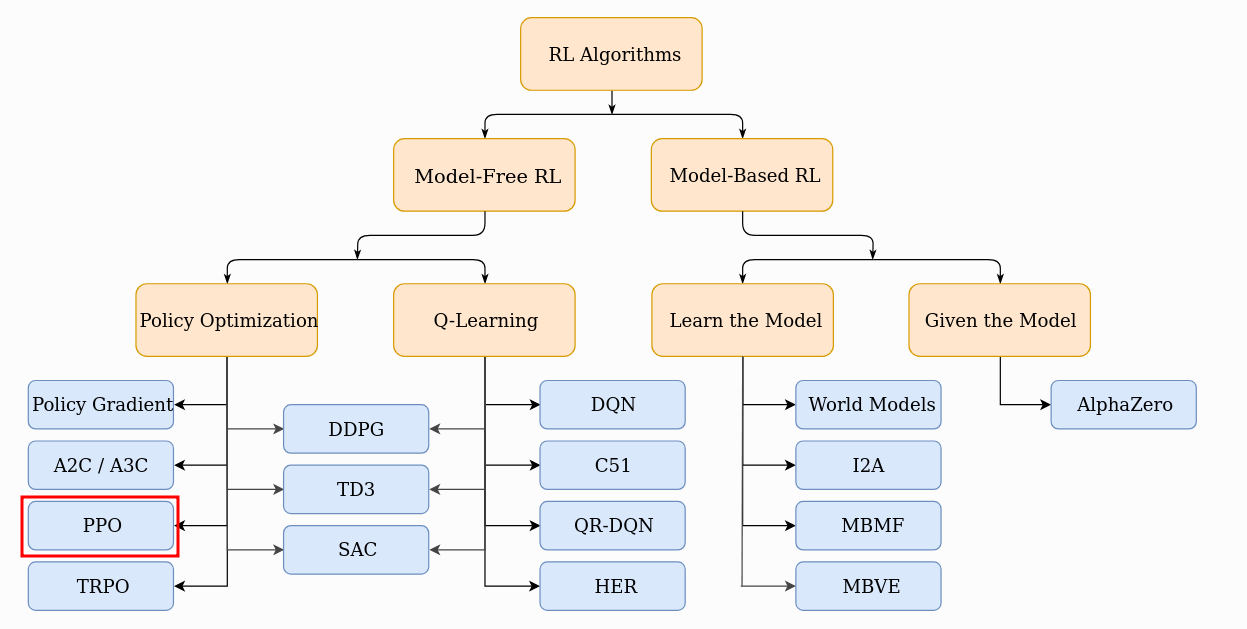
\includegraphics[width=0.8\textwidth]{components/algorithm_selection.png}
		\caption{ \textit{RL algorithm classification} src: \cite{openaispin}}
		\label{fig:algorithm_selection}
	\end{center}
\end{figure}


As mentioned in custom environment section above, the action to be performed by an agent is the bidirectional charging and discharging power of a battery storage system on a continuous series of observation, an algorithm with continuous action space is selected. Based on policy learning type on whether to use the sample collection and simultaneous learning(i.e. on-policy) or to used sample collection and learn from them separately (i.e. off-policy), algorithms of both type were considered. \\


Based on state spaces exposed to the agent, the observable space is only partial. Since the full dynamics of environment are not known beforehand, model-free algorithms are considered for their simplicity and effectiveness. Considering above described criteria, policy gradient based algorithm Proximal Policy Optimization(PPO) \cite{ppo}, Soft Actor Critic(SAC)\cite{sac}, and Twin Delayed Deep Deterministic Policy Gradient(TD3)\cite{td3} were selected from \cite{sb3} for the experiments. \\

A partial but crucial component of the algorithm is an actor network that predicts action given the set of observation. The actor network is part of in each all the selected algorithms. A typical architecture of an actor network is shown in figure \ref{fig:actor_network}. Given observation inputs of Power household, Power PV, Energy exchange price and current battery SoC, action is the resultant of an Fully connected Multi Layer Perceptron(FC-MLP), with appropriate activation $Z$(hyperbolic tangent due to it's compatibility with action space $A \in [-1,1]$). \\

\begin{figure}[h]
	\begin{center}
		\includegraphics[width=\textwidth]{components/actor_network.png}
		\caption{ \textit{Actor (pi) network}}
		\label{fig:actor_network}
	\end{center}
\end{figure}


Modeling a Prosumer Agent for selected algorithms effectively for the application under consideration, evaluating performance and identifying different factors influencing the learning of better strategies is the main focus of this undertaking. The briefed methodologies above guide the development of experimental setup in the following section \ref{ch-3}. \\

To bring the components together, steps of procedure is to be outlined for development. Following the definition of custom environment and their types, selected algorithms, relevant system states are defined. An action boundary, constraining agents action to operational range of a battery system is to be setup. A mapping of system states to resulting action is in accordance with the selected algorithms for learning policies. Starting from randomly initialized policy and criteria defining reward estimation, an appropriate behavior is modeled via the interaction of environment and policy learning algorithms.  An agent is evaluated based on actions that optimizes the household net cost of exchange to a grid under variable tarrifs and improved based on the reward feedback. This iterative policy learning, evaluation and improvement process is expected to derive policy toward optimality. \\ 


\end{large}
% ------------------------------------------------------------------------------------



\chapter{Development} \label{ch-3}

% ------------------------------------------------------------------------------------
\begin{large}
	
In order to experiment and collect observations on agents experience, implementation of different components defined in previous section, preparation of observation inputs, training of agents, iterative evaluation and improvement, taking feedback from different stages and re-training under set of parameter configuration, a pipeline is outlined based on flow of information as shown in figure \ref{fig:dev_pipeline}. Following subsections describe each component of the pipeline in detail.


\begin{figure}[h]
	\begin{center}
		\includegraphics[width=0.9\textwidth]{development/pipeline.png}
		\caption{ \textit{Development pipeline} }
		\label{fig:dev_pipeline}
	\end{center}
\end{figure}

Scoping defines development criteria for environment components, initialization parameters, metrics to track for the model performance and define a comparable baseline based on rule-based conditionals. Data processing step involves extraction, transformation, and merging dataset to prepare observation inputs for the environment. Train-evaluation involves steps required for modeling of a policy and saving intermediate/final results for inference. Testing involves sampling of action from the saved policy. Final step involves export of saved policy and sets up a prototypical scenario for a real world HEMS control.

\section{Scoping}

Based on the objectives identified and research question discussed in introduction section, the scope for environment development, selection of features, modeling of policies and sample testing from a modeled policy is determined. The custom environment setup requires definition of observation and action space, step function for step transition in the environment, definition of reward objective, and resetting methods for every time environment step is initiated(i.e. resetting states to initial state). Following list outlines scoping of components \\

\begin{itemize}
	\item \textbf{Observation space}: range of each observation input features is scoped within the maximum and minimum values of the series, defining upper and lower bounds respectively. 
	\item \textbf{Action space}: similar to observation space, action space is defined, i.e. $a \in (-11, 11) \forall a \in A$. During implementation the range is set to $(-1, 1)$ and is later scaled during step transition in an environment to reduce computational complexity.
	\item \textbf{Optimization objective}: Main objective is to minimize cost using a power balance equation by computing the net exchange to the grid and applying exchange rate prices \ref{eq:costreward}. Additional objectives are battery care or retain of soc by rewarding desired threshold and discouraging when out of range as defined in equation \ref{eq:combinedreward} of methodology section.
	\item \textbf{Metrics to track}: evaluation of performance of a model based on reward objectives during training are defined in terms of accumulation of mean episodic rewards representing the net exchange cost.
	\item \textbf{Rule based Baseline}: in order to measure the relative performance of a given policy, a rule based policy is set as a baseline. Although the actions in rule based scenario are discrete and pre-defined in contrast to action predicting learned policies, it provides a rough cost comparison among policies. The detail pseudo code is described in the following section.
	
	\item \textbf{RL based Algorithms}:
\end{itemize}

\section*{Rule-based Strategy}

\begin{lstlisting}
for length 'i' of test observation window:
  exchange = power_pv[i] + power_household[i]
  if exchange < 0:  # excess pv
    if battery.current_soc == 1: 
      net_exchange = exchange + action # feed into grid
    else:
      action = max_charge_rate  # charge
  else:
    if battery.current_soc == 0:
      net_exchange = exchange + action # draw from grid
	else:
	  action = max_discharge_rate # discharge
\end{lstlisting}

\section*{RL based Algorithms}

PPO is an on-policy algorithm with improvement on Trust Region Policy Optimization(TRPO) \cite{trpo} and mainly deals with large update in policy, so that it does not collapse. TRPO uses KL divergence to define this constraint. PPO uses clipping based objective to achieve this constraint. Figure \ref{fig:ppo_pseudocode} shows the steps involved in learning of the policy network. Initialized with random parameters $\theta$ of for policy network and value network parameters $\phi$, it collects agents experience under policy $\pi$ and uses Stochastic Gradient Accent(SGA) to maximize clip based objective and Stochastic Gradient Descent(SGD) to minimize the value error. 

\begin{figure}[h]
	\begin{center}
		\includegraphics[width=\textwidth]{components/ppo_pseudocode.png}
		\caption{ \textit{Pseudo code for PPO}}
		\label{fig:ppo_pseudocode}
	\end{center}
\end{figure}

TD3 is off-policy algorithm based on improvement of shortcomings in  Deep Deterministic Policy Gradient(DDPG)\cite{ddpg}, of overestimating Q values leading to policy degradation. TD3 introduces identical Q-value estimators as targets with delay and policy smoothing techniques. The learning of a policy network is done by computing target Q functions and updating the parameters of using  gradient ascent and using the least of these two values mitigating overestimation as shown in figure \ref{fig:td3_pseudocode} \\

\begin{figure}[h]
	\begin{center}
		\includegraphics[width=\textwidth]{components/td3_pseudocode.png}
		\caption{ \textit{Pseudo code for TD3}}
		\label{fig:td3_pseudocode}
	\end{center}
\end{figure}

SAC is also an off-policy algorithm which uses double Q-functions as targets and policy smoothing techniques similar to TD3. It introduces entropy terms in the target networks for exploration and alternatively updates parameter using gradient descent for Q-function and gradient ascent for policy network parameters. A detailed pseudo-code for SAC is shown in figure \ref{fig:sac_pseudocode} \\


\begin{figure}[h]
	\begin{center}
		\includegraphics[width=\textwidth]{components/sac_pseudocode.png}
		\caption{ \textit{Pseudo code for SAC}}
		\label{fig:sac_pseudocode}
	\end{center}
\end{figure}


\section{Data Processing: Extract, Transform and Load(ETL)}

The dataset from two different Prosumers(alias p1 and p2), containing data within time frame($2021-2022$) were used. This dataset then go through series of transformation before it is initialized within an environment as observation inputs. These transformations include combination of household and auction price dataset by concatenation, aligning and transforming sample timesteps and frequency, unit conversion and handling of missing or outlying values as shown in figure \ref{fig:dev_dataetl}. The resulting dataset is of length $70082$ including p1 and p2 each containing $35041$ entries with time index range of \textit{2021-08-15 00:00} to \textit{2022-08-15 00:00} UTC. \\

\begin{figure}[h]
	\begin{center}
		\includegraphics[width=0.9\textwidth]{development/dataetl.png}
		\caption{ \textit{Data Pre-processing} }
		\label{fig:dev_dataetl}
	\end{center}
\end{figure}


\section{Modeling: Policy Train-Evaluation Iteration}

This step includes implementation of setup for learning parameters of a policy network, evaluation of performance and freezing of parameter saved as checkpoint for every step of policy evaluation-improvement iteration as shown with simplification in figure \ref{fig:dev_train_eval}. Modeling in this context refers to the optimization of policy network parameters toward the ones resulting in near intended actions. \\

Training part of the iteration begins with a policy network with randomly initialized internal parameters. These parameters are updated for $i$ number of iteration in a train environment and are evaluated in an evaluation environment. An evaluation step involves $j$ number of episodes and taking an average to calculate the score. After evaluation the parameters are saved as checkpoint. The goal is to maximize this score for each passing iteration using gradient assent to update parameters. The rate of update is defined by learning rate. The iteration of training continues untill the end of specified number of train cycle with continuous evaluation score returns. Retraining involves same steps except for starting from a randomly initialized policy, it must start with checkpoint of a policy that was previously trained. The rest of the step are identical, and one could either train or retrain at a time. \\

\begin{figure}[h]
	\begin{center}
		\includegraphics[width=0.9\textwidth]{development/train_eval.png}
		\caption{ \textit{Train-evaluation iteration} }
		\label{fig:dev_train_eval}
	\end{center}
\end{figure}

\section{Policy Testing}

This steps is completely separate from training and evaluation as it uses input observation that are not used during training in a dedicated test environment. The policy network is loaded with the updated and saved parameters form the training-evaluation iteration. Test input observation are then passed through the actor network resulting in predicted action. This action is used to compute net exchange, update battery SoC and finally to calculate total cost of net exchange per episode as described in the section \ref{ch-2}. \\

\begin{figure}[h]
	\begin{center}
		\includegraphics[width=0.9\textwidth]{development/testing.png}
		\caption{ \textit{Testing of Trained Policy} }
		\label{fig:dev_test}
	\end{center}
\end{figure}

\section{Model Export}

This step involves export of trained model to be used as a controller outside of the simulated HEMS environment. The models exported checkpoints saved as a compressed .zip format from modeling, are converted to pytorch format by extracting the Actor network, since it is responsible for action prediction, the critic network is discarded. The saved pytorch format checkpoint are further converted to open onnx format, which can be used for serving the model using various platforms. The model are then served through api endpoints to return the action given set of observations. The model server module, written in Flask, is containerized for further deployment.  \\


The pipeline, following the methodology, starting from conceptual scoping to sample deployment, concludes the part of development. The checkpoints from the testing section above are used to sample actions for novel set of testing set for each algorithms and observations are visualized in the next section. \\
	
\end{large}
% ------------------------------------------------------------------------------------
\chapter{Observations} \label{ch-4}

\begin{large}

This section reports the observed results, during training, testing and derived net grid exchange cost from action sampled given trained policy. The dataset was split into training and test set with the ratio of 90\% and 10\% respectively. The custom environment was setup in such a way that it takes window of observation input of $2$ weeks length and shuffles the train set uniformly randomly to get different set of input observation for next iteration. Discount factor for the model were kept $0.99$ for all models\\

\section{Parameters}

There exists plethora of combination of hyper-parameters that can be searched and tested further to improve current policy. List \ref{lst:params} shows a set of model hyper-parameter settings under which the observations are collected during training and testing of the policy.\\

\begin{lstlisting}
env_observation_window_train=int(24 * 4 * 7 * 2)
policy_nw="MlpPolicy"
num_train_eval_cycles=200
num_eval_episodes_per_cycle=2
num_test_episodes=5
train_timesteps=env_observation_window_train * 2
ppo_learning_rate=0.0003
ppo_clip_range=0.20
ppo_nws={"pi": [64, 64, 16], "vf": [64, 64, 16]} 
sac_learning_rate=0.0003
sac_tau=0.005
sac_nws={"pi": [256, 256, 16], "qf": [256, 256, 16]}
td3_learning_rate=0.001
td3_tau=0.005
td3_nws={"pi": [128, 128, 16], "qf": [128, 128, 16]}
\end{lstlisting}


\section{Observation during Train/Evaluation Cycle}

Observation were recorded for optimization of perceived cost per episode for constant and variable auction price as described in the section below. A combined objective was also recorded with cost based reward and reward for retaining fraction of SoC in a battery. Observations for the combined objective are included as part of supplementary observation \ref{ch-5} \\

\subsection*{With constant exchange rate}

The performance of a policy during training is measured using the cost optimized by each algorithm. The networks were each trained for $200$ cycle of training and for each training, $2$ iteration of evaluation was performed and average was taken as a performance score for that iteration. The metrics recorded and visualized for optimization under constant tariff for grid feed and draw rate of $0.08$ and $0.33$ Eur/kWh respectively as shown in figure \ref{fig:cost_compare_constant_ap}. \\

% with constant auction price
\begin{figure}[h]
	\begin{center}
		\includegraphics[width=0.9\textwidth]{observation/constant_ap/comparison_ppo_sac_td3.png}
		\caption{ \textit{Cost reward evaluation per episode with constant auction price} }
		\label{fig:cost_compare_constant_ap}
	\end{center}
\end{figure}

% retrained ppo
\begin{figure}[h]
	\begin{center}
		\includegraphics[width=0.9\textwidth]{observation/constant_ap/comparison_ppo_retrain.png}
		\caption{ \textit{Cost reward evaluation per episode with retrained PPO} }
		\label{fig:cost_compare_constant_ap_ppo_retrain}
	\end{center}
\end{figure}

With perceived saved cost in relation to number of train-evaluation cycle, the comparison of cost is higher for TD3, SAC has more consistency over all with early positive trend. The PPO however is fluctuating and does not seem to plateau until the end of $200^{th}$ cycle. Upon further retraining for $200$ more cycles, it is improved, showing consistent value as shown in the figure \ref{fig:cost_compare_constant_ap_ppo_retrain}. One of the reason for PPO to learn relatively slowly is due to the slow update of the network parameters based on sample collected under current policy, since it is on-policy algorithm. In contrast, TD3 and SAC which are off-policy therefore more sample efficient. \\

\subsection*{With variable exchange rate}

The same cost based metrics were tracked for comparison with variable auction price dataset. Unlike under constant exchange rate price the feed in and draw from the grid is a same rate. The evaluated perceived cost saving per episode for variable auction price is shown in figure \ref{fig:cost_compare_variable_ap} \\ 


% with variable auction price
\begin{figure}[h]
	\begin{center}
		\includegraphics[width=0.9\textwidth]{observation/variable_ap/comparison_ppo_sac_td3.png}
		\caption{ \textit{Cost reward evaluation per episode with variable auction price} }
		\label{fig:cost_compare_variable_ap}
	\end{center}
\end{figure}

The PPO is retrained also in the case of model with variable exchange cost and shows improvements after $200^{th}$ iteration. Although there seems to be a small trend at the end of the $200$ cycle of retraining and evaluation, no further training was done. The retrained ppo with evaluation score is shown in figure\ref{fig:cost_compare_ap_ppo_retrain} \\

% retrained ppo
\begin{figure}[h]
	\begin{center}
		\includegraphics[width=0.9\textwidth]{observation/variable_ap/comparison_ppo_retrain.png}
		\caption{ \textit{Cost reward evaluation per episode with retrained PPO} }
		\label{fig:cost_compare_ap_ppo_retrain}
	\end{center}
\end{figure}

\section{Observation during Testing}

This section shows an agents experience on untrained dataset. In correspondence to the scenario of constant and variable auction price discussed in observation during training, the performance of a model was calculated for observation input window of A week(24*4*7 time steps). In addition, for the same window cost is computed for rule based strategy for comparison. \\

\subsection*{with Constant Exchange rate}

The experience of an agent under constant auction price for rule based strategy can be seen in figure \ref{fig:test_compare_constant_ap_rbc}. The effect of variable PV generation directly corresponds to the action(i.e. charging during pv generation) and consequent change in battery SoC. \\

% rbc
\begin{figure}[h]
	\begin{center}
		\includegraphics[width=0.9\textwidth]{observation/constant_ap/rbc/rbc_comparison.png}
		\caption{ \textit{Rule based policy with constant auction price} }
		\label{fig:test_compare_constant_ap_rbc}
	\end{center}
\end{figure}

% td3
\begin{figure}[h]
	\begin{center}
		\includegraphics[width=0.9\textwidth]{observation/constant_ap/td3/test/td3_rbc_comparison.png}
		\caption{ \textit{TD3 with constant auction price} }
		\label{fig:test_compare_constant_ap_td3}
	\end{center}
\end{figure}

RL based agent with TD3 under the same scenario of constant auction price is shown in figure \ref{fig:test_compare_constant_ap_td3}. The reflection of variable PV generation corresponds to small change in action and the SoC however, the average cost saving in higher. Looking into the grid exchange component in the subplot, the agent has learned to save cost by selling  all the energy back to the grid, as indicated by the negative grid exchange . \\

\begin{table}
	\begin{center}
		\begin{tabular}{ccccc} 
			\hline % -------------------------------------------------------------
			\vspace{0.5pt} \\
			\textbf{Model Config} & \textbf{PPO} & \textbf{SAC} & \textbf{TD3} & \textbf{RBP} \\ % Header
			\hline % -------------------------------------------------------------
			\vspace{0.5pt} \\
			\textbf{Untrained} & 54.405 & 54.417  & 54.405 & 0.0 \\
			\textbf{Constant AP} & 242.696 & 255.239  & \textbf{314.556}  & 312.382 \\
			\textbf{Constant AP with PPO retrained} & 272.971 & -  & -  & - \\
			\hline % -------------------------------------------------------------
		\end{tabular}
		\caption{Comparison per policy with constant exchange rate }
		\label{table:comparison_constant_ap} % Label for referencing the table 
	\end{center}
\end{table}

Comparison of cost based score for RL based and Rule based methods is shown is the table \ref{table:comparison_constant_ap}. TD3 model has learned to optimize the cost more effectively than the other RL based algorithm and slightly better than the rule based strategy. \\  

% rbc
\begin{figure}[h]
	\begin{center}
		\includegraphics[width=0.9\textwidth]{observation/variable_ap/rbc/rbc_comparison.png}
		\caption{ \textit{Rule based policy with variable auction price} }
		\label{fig:test_compare_variable_ap_rbc}
	\end{center}
\end{figure}

\subsection*{with Variable Exchange rate}

With variable auction price as part of observation input, rule based strategy has similar results as shown in figure \ref{fig:test_compare_variable_ap_rbc}. Since the exchange rate has changed and there is no complex modeling of variability, the change is apparent only in the net cost of exchange computation relative to rbc with constant price. \\ 

% sac energy 
\begin{figure}[h]
	\begin{center}
		\includegraphics[width=0.9\textwidth]{observation/variable_ap/sac/test/sac_rbc_comparison.png}
		\caption{ \textit{SAC with variable auction price} }
		\label{fig:test_compare_variable_ap_sac}
	\end{center}
\end{figure}

As shown in the figure \ref{fig:test_compare_variable_ap_sac}, SAC has learned to optimize it behavior based on variable auction price as well with the spike in charging action, when the energy cost is $0$ and discharges immediately when the exchange price is higher. In rest of the cases it chooses to sell all the energy for cost profit, since there is no constraint, neither incentive on keeping the energy. \\

\begin{table}
	% ------------------------------------------------------------------------------
	\begin{center}
		\begin{tabular}{ccccc} 
			\hline % -------------------------------------------------------------
			\vspace{0.5pt} \\
			\textbf{Model Config} & \textbf{PPO} & \textbf{SAC} & \textbf{TD3} & \textbf{RBP} \\ % Header
			\hline % -------------------------------------------------------------
			\vspace{0.5pt} \\
			\textbf{Untrained} & 91.371 & 91.371  & 91.371  & 0.0 \\
			\textbf{Variable AP} & 459.578 & \textbf{601.228}  & 297.622  & 140.857 \\
			\textbf{Variable AP wit PPO retrained} & 453.212 & -  & -  & - \\
			\hline % -------------------------------------------------------------
		\end{tabular}
		\caption{Comparison of performance per policy with variable exchange rate}
		\label{table:comparison_variable_ap} % Label for referencing the table 
		
	\end{center}
\end{table}

Table \ref{table:comparison_variable_ap} shows the comparison score with significant improvement of RL based algorithms, specially with SAC, taking advantage of variable exchange price, selling all possible energy to maximize the profit. Rule based strategies however has slightly lower score than with the case of constant auction price. \\

With simple rule-based strategy as a baseline and score of randomly initialized untrained policy as a comparison criteria, improvement can be seen in each case whether under constant or variable exchange price. \\

\section{Discussion}

%expectation vs outcomes ...

There were some improvement that were challenging to address in the implementation setup used to collect observation, mainly design of reward function. It was several time updated back and forth to include and improve the objectives. The combination, as in the case with retaining SoC were resulting in poor observations. The improvement achieved in this combined part is included as supplementary observation \ref{ch-6}. The results are better than random policy but in combination with cost optimization objective simultaneously not as much. Multi-objective frameworks are likely suitable to mitigate this issue. \\

In addition, there were several experimentation and efforts that were made to stabilize and improve the modeling and observation of the Policy. Searching of hyper-parameters were conducted with the use of optimization libraries however, the search trial were based on running the experiment for couple of episode to calculate score. In practice there were runs that even after 100 of episodes suddenly drop their performance to close to initial policy. This led to manual trial and error starting with default values and changing and observing the results. \\

In general most of the investment were made for iterative  implementation, change and experimentation of different components. 

\end{large}



\unnumberedchapter{Conclusion}
\chapter*{Conclusion and Further Work} \label{ch-5}  % Name of the unnumbered section
% ------------------------------------------------------------------------------------
\begin{large}

\vspace*{3\baselineskip}

This work primarily focused on exploration and usage of RL based methods to find control strategies within a Prosumer household in an effort to minimize cost of energy usage. \\

To address the first research question of how a Prosumer agent is modeled using RL, an experimental platform was implemented using customized simulated HEMS environment and through iterative evaluation and improvement, policy for an Agents actions were modeled. The second question of effective minimization of cost of energy under time-variable tariffs was demonstrated by the test of the agents policy on unseen set of inputs as shown in \ref{table:comparison_variable_ap}. To test out the choice of algorithm and it's impact on performance and efficiency of the control system was also demonstrated with exploration algorithm that are on and off-policy. The off-policy algorithms TD3 and SAC are perfoming better in each of the three scenarion of cost optimization under constant energy exchange price, under variable exchange price  and combined objective under variable price with fractional soc retain. Finally, the key factors influencing the optimal control strategies were identified as the selection of RL algorithm, usage of suitable parameters such as size of observation window, number of hidden layers and number of hidden layer in each unit of the Actor, Value and Q network, and contribution of other model specific parameters such as reward discounting, constraint on policy update. Since small change in value of one parameter causes drastic change in behavior of RL based agent due to the sensitivity  of these algorithms, it is often the case of trial and improvement as in the case of most of deep neural network based algorithm. \\

In conclusion, this work demonstrates progressive improvement in performance of RL algorithm, starting from randomly initialized network, learning in different set of observation input setting and performing with significant score on the defined objective. \\

Further improvement can be made to include multi objective reward optimization, searching for more optimal parameters and inclusion of more input features and separate action space for EVSE and Household battery charger.

\end{large}
% ------------------------------------------------------------------------------------

\unnumberedchapter{Supplementary Observations}
\chapter*{Supplementary Observations} \label{ch-6} % Name of the unnumbered section
% ------------------------------------------------------------------------------------
\begin{large}
\vspace*{3\baselineskip}

This is a supplementary section including optimization of multiple objectives of minimizing the net cost and retain $45\%$ of the battery soc. The observation of performance of policy during training and testing is described in this section. To retain defined amount of SoC during policy learning was implemented by encouraging the agent with the value of $0.25$, if it keeps the SoC value above $45\%$ and $-0.25$ otherwise. This value is added to the cost reward to obtain the final reward. \\

\section*{Combined Reward Optimization (cost with soc retain)}

The performance of a policy of all the model based on cost reward and combined reward is shown in figure \ref{fig:comparison_ppo_sac_td3_cost_soc_retain} and \ref{fig:comparison_ppo_sac_td3_combined_soc_retain} respectively. It is clear from these figures, the agent is maximizing the combined reward with higher emphasis because it achieves maximum value of around $800$. On the other hand the cost based reward only achieves maximum value around $115$. Since there is no rule based comparison for multiple rewards, the rl based models are compared among themselves by referencing the score during initialization. \\

\begin{figure}[h]
	\begin{center}
		\includegraphics[width=0.9\textwidth]{observation/soc_retain/comparison_ppo_sac_td3_cost.png }
		\caption{ \textit{Cost reward evaluation per episode with variable auction price and soc retain} }
		\label{fig:comparison_ppo_sac_td3_cost_soc_retain}
	\end{center}
\end{figure}

The combined reward value has no significance by itself like cost based reward which is calculated with the energy balance equation described by \ref{eq:costreward} and actually represents net exchange cost. The combined reward dominates the cost reward with the soc retain reward value of  $\pm0.25$. Decreasing this value retains less to no soc and increasing the value only increases the combined reward at the expense of cost reward. \\

\begin{figure}[h]
	\begin{center}
		\includegraphics[width=0.9\textwidth]{observation/soc_retain/comparison_ppo_sac_td3_combined.png }
		\caption{ \textit{Combined reward evaluation per episode with variable auction price and soc retain} }
		\label{fig:comparison_ppo_sac_td3_combined_soc_retain}
	\end{center}
\end{figure}

While testing of the learned policy reinforced by this combined reward, each model retains the desired amount but the cost optimization is hindered as shown in the table \ref{table:comparison_variable_ap_soc_retain} \\

% sac
\begin{figure}[h]
	\begin{center}
		\includegraphics[width=0.9\textwidth]{observation/soc_retain/sac/test/sac_rbc_comparison.png}
		\caption{ \textit{Agents sample action from SAC policy with variable auction price and soc retain}}
		\label{fig:test_compare_soc_retain_sac}
	\end{center}
\end{figure}

% td3
\begin{figure}[h]
	\begin{center}
		\includegraphics[width=0.9\textwidth]{observation/soc_retain/ppo/test/ppo_rbc_comparison.png}
		\caption{ \textit{Agents sample action from PPO policy with variable auction price and soc retain}}
		\label{fig:test_compare_soc_retain_ppo}
	\end{center}
\end{figure}

The figures \ref{fig:test_compare_soc_retain_sac}, \ref{fig:test_compare_soc_retain_ppo} show that, regardless of hindrance in average cost minimization, both policies show some pattern of reflected variability in the observation input for SAC and PPO respectively. The patterns are most visible in SAC, which resonates with the relatively higher value than other RL based strategies. The TD3 has barely improved on from the random state of initialization. \\

Overall, these observations show that the objective of retaining SoC is met, but the average cost of exchange is not minimized, indicating that the improvement in cost contribution could be made with searching for better definition of reward function and balanced composition of combined rewards constituents. \\

\begin{table}
	% ------------------------------------------------------------------------------
\begin{center}
	\begin{tabular}{ccccc} 
		\hline % -------------------------------------------------------------
		\vspace{0.5pt} \\
		\textbf{Model Config} & \textbf{PPO} & \textbf{SAC} & \textbf{TD3} \\ % Header
		\hline % -------------------------------------------------------------
		\vspace{0.5pt} \\
		\textbf{Untrained} & 91.371 & 91.371  & 91.371 \\
		\textbf{Variable AP and SoC retain} & 98.325 & \textbf{109.296}  & 93.987 \\
		\hline % -------------------------------------------------------------
	\end{tabular}
	\caption{ comparison per policy with variable exchange rate}
	\label{table:comparison_variable_ap_soc_retain}
	
\end{center}
\end{table}
	
\end{large}
% ------------------------------------------------------------------------------------

\unnumberedchapter{List of Figures and Tables}
\chapter*{List of Figures and Tables} \label{ch-7}  % Name of the unnumbered section
% ------------------------------------------------------------------------------------
\begin{large}
\vspace*{3\baselineskip}

\section*{Figures}

\begin{itemize}
	\item Energy generation in Germany per year [2002-2023] \ref{fig:energy_gen_de}
	\item Data distribution of observation inputs \ref{fig:dev_datainfo}
	\item Additive decomposition of observation inputs (daily) \ref{fig:dev_input_decompose_daily}
	\item Additive decomposition of observation inputs (hourly) \ref{fig:dev_input_decompose_hourly}
	\item {Agent environment interaction} \ref{fig:fmdp}
	\item Custom simulated HEMS environment \ref{fig:custom_env}
	\item Types of environments \ref{fig:env_types}
	\item Actor (pi) network \ref{fig:actor_network}
	% Development pipeline
	\item Development pipeline \ref{fig:dev_pipeline}
	\item Data Pre-processing \ref{fig:dev_dataetl}
	\item Train-evaluation iteration \ref{fig:dev_train_eval}
	\item Testing of Trained Policy \ref{fig:dev_test}
	% Observations
	\item Cost reward evaluation per episode with constant auction price \ref{fig:cost_compare_constant_ap}
	\item Cost reward evaluation per episode with retrained PPO \ref{fig:cost_compare_constant_ap_ppo_retrain}
	\item Cost reward evaluation per episode with variable auction price \ref{fig:cost_compare_variable_ap}
	\item Cost reward evaluation per episode with retrained PPO \ref{fig:cost_compare_ap_ppo_retrain}
	\item Rule based policy with constant auction price \ref{fig:test_compare_constant_ap_rbc}
	\item TD3 with constant auction price \ref{fig:test_compare_constant_ap_td3}
	\item Rule based policy with variable auction price
	\ref{fig:test_compare_variable_ap_rbc}
	\item SAC with variable auction price \ref{fig:test_compare_variable_ap_sac}
\end{itemize}

\section*{Tables}	

\begin{itemize}
	% Observations
	\item Comparison per policy with constant exchange rate
	\ref{table:comparison_constant_ap}
	\item Comparison of performance per policy with variable exchange rate \ref{table:comparison_variable_ap}
\end{itemize}


\end{large}
% ------------------------------------------------------------------------------------

% Bibliography
% ............................................................................

\begin{thebibliography}{9}

\begin{large}
% ------------------------------------------------------------------------------------

\bibitem{parisagreement} The Paris Agreement. (2015). \emph{UN Climate Change Conference}

\bibitem{climateact}  Climate Change Act, Intergenerational contract for the climate. (2021). \emph{Die bundesregierung, Energie und Klimaschutz.} 

\bibitem{energychartsinfo} Energy charts info. (2024). \emph{www.energycharts.info}.

\bibitem{sems} Moen, Roger. Solar energy management system. (1979). \emph{IEEE, $18^{th}$ Conference on Decision and Control}. 

\bibitem{evess} Mohammad et al. (2021). Integration of Electric Vehicles and Energy Storage System in Home Energy Management System with Home to Grid Capability. \emph{Energies 2021, 14, 8557}

\bibitem{milp} Hou et al. (2019). Smart Home Energy Management Optimization Method Considering ESS and PEV. \emph{ICIEA} 

\bibitem{dphev} ZHU et al. Optimization of rule-based energy management strategies for hybrid vehicles using
dynamic programming. (2021). \emph{Combustion Engines.}


\bibitem{qlearning}Lee et al. (2019). Reinforcement Learning-Based Energy Management of Smart Home with Rooftop Solar Photovoltaic System, Energy Storage System, and Home Appliances. \emph{ensors (Basel). 2019 Sep 12;19(18):3937}

\bibitem{drlgym}Specht et al. (2023) Deep reinforcement learning for the optimized operation of large amounts of distributed renewable energy assets. \emph{Energy and AI 11 (2023) 100215}

\bibitem{dataset} Ostermann et al, (2023). \emph{Bidirectional Electric Vehicles Field Trial Data Set}, NEIS 2023.

\bibitem{rlintro}Sutton et al. (2018). \emph{Reinforcement learning: An introduction} (2nd ed.). The MIT Press.

\bibitem{openaispin} OpenAI: Spinning Up in Deep Reinforcement Learning. (2018).

\bibitem{ppo}Schulman et al. (2017). \emph{Proximal Policy Optimization Algorithms}. arXiv:1707.06347v2.

\bibitem{sac}Tuomas et al. (2018). \emph{Soft Actor-Critic: Off-Policy Maximum Entropy Deep Reinforcement Learning with a Stochastic Actor}. arXiv:1801.01290v2.

\bibitem{td3}Fujimoto et al. (2018). \emph{Addressing Function Approximation Error in Actor-Critic Methods}. arXiv:1802.09477v3.

\bibitem{sb3}Raffin et al. (2021). \emph{Stable-Baselines3: Reliable Reinforcement Learning Implementations}. Journal of Machine Learning Research.

\bibitem{gymnasium}Towers et al. (2023). \emph{Gymnasium, An API standard for single-agent reinforcement learning environments}. Zenodo.

\bibitem{trpo}Schulman et al. (2017). Trust Region Policy Optimization \emph{arXiv:1502.05477v5}.

\bibitem{ddpg}Lillicrap et al. (2019). Continuous control with deep reinforcement learning. \emph{arXiv:1509.02971v6}.

\end{large}
% ------------------------------------------------------------------------------------

 
\end{thebibliography}

\end{document}

% ----------------------------------------------------------------------------
% End of Document
% ----------------------------------------------------------------------------
